\documentclass{beamer}
\usefonttheme{serif}
\usepackage{graphicx}
\usepackage{amsmath}
\usepackage{hyperref}



\iffalse

\fi

\title{Birdsong identification with Convolutional Neural Networks}
\author{Eduardo Quintana Miranda}

\begin{document}

\frame{\titlepage}

\begin{frame}
    \begin{figure}\
        \centering{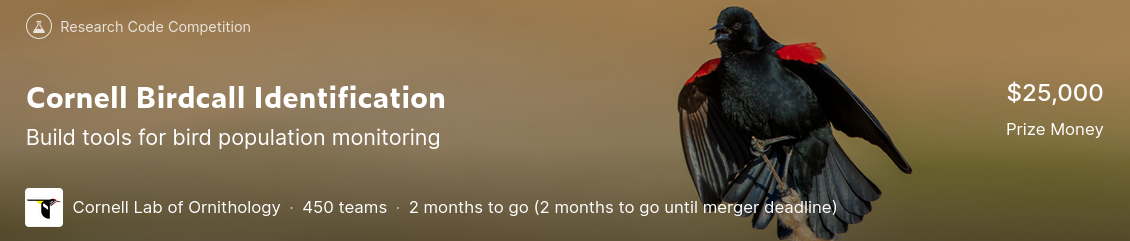
\includegraphics[width=\textwidth]{images/kaggle.png}}
        \centering{\hbox{\url{https://www.kaggle.com/c/birdsong-recognition}}}
    \end{figure}
    \begin{itemize}
        \item 264 bird classes,
        \item 21'000 audio files (16 hours total),
    \end{itemize}
\end{frame}

\begin{frame}
    \newlength{\picwidth}
    \setlength{\picwidth}{.2\textwidth}
    \centering{
    \begin{tabular}{cccc}
        \vbox{%
        \hbox{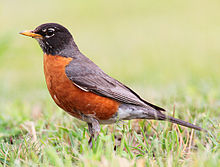
\includegraphics[width=\picwidth]{images/amerob.jpg}}
        \hbox{\tiny American robin}}
        & 
        \vbox{%
        \hbox{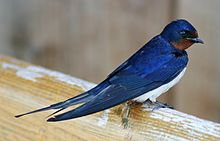
\includegraphics[width=\picwidth]{images/barswa.jpg}}
        \hbox{\tiny Barn swallow}}
        & 
        \vbox{%
            \hbox{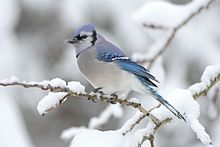
\includegraphics[width=\picwidth]{images/blujay.jpg}}
            \hbox{\tiny Blue jay}}
        & 
        \vbox{%
            \hbox{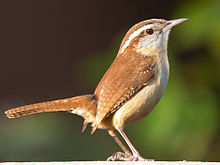
\includegraphics[width=\picwidth]{images/carwre.jpg}} 
            \hbox{\tiny Carolina wren}}
            \\
        \vbox{%
            \hbox{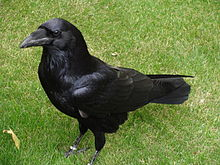
\includegraphics[width=\picwidth]{images/comrav.jpg}}
            \hbox{\tiny Common raven}}
        & 
        \vbox{%
            \hbox{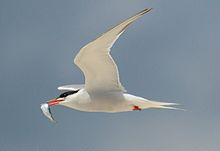
\includegraphics[width=\picwidth]{images/comter.jpg}}
            \hbox{\tiny Common tern}}
        & 
        \vbox{%
            \hbox{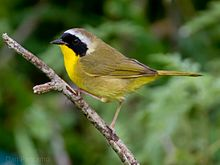
\includegraphics[width=\picwidth]{images/comyel.jpg}}
            \hbox{\tiny Common yellowthroat}}
        & 
        \vbox{%
            \hbox{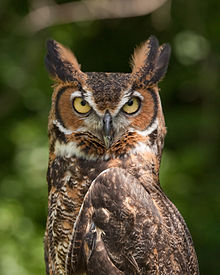
\includegraphics[width=\picwidth]{images/grhowl.jpg}}
            \hbox{\tiny Great horned owl}}
            \\
        \vbox{%
            \hbox{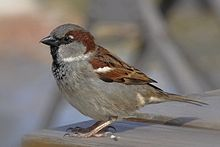
\includegraphics[width=\picwidth]{images/houspa.jpg}}
            \hbox{\tiny House sparrow}}
        & 
        \vbox{%
            \hbox{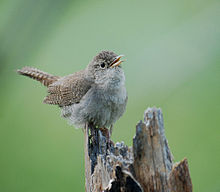
\includegraphics[width=\picwidth]{images/houwre.jpg}}
            \hbox{\tiny House wren}}
        &
        \vbox{%
            \hbox{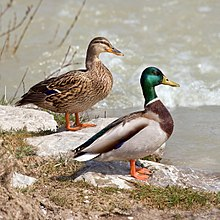
\includegraphics[width=\picwidth]{images/mallar3.jpg}}
            \hbox{\tiny Mallard}}
        & 
        \vbox{%
            \hbox{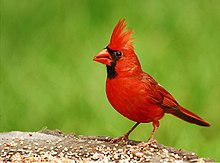
\includegraphics[width=\picwidth]{images/norcar.jpg}}
            \hbox{\tiny Northern cardinal}}
            \\
        \vbox{%
            \hbox{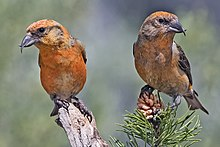
\includegraphics[width=\picwidth]{images/redcro.jpg}}
            \hbox{\tiny Red crossbill}}
        & 
        \vbox{%
            \hbox{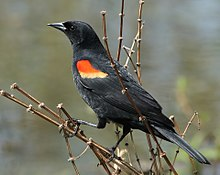
\includegraphics[width=\picwidth]{images/rewbla.jpg}}
            \hbox{\tiny Red-winged blackbird}}
        &
        \vbox{%
            \hbox{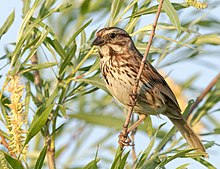
\includegraphics[width=\picwidth]{images/sonspa.jpg}}
            \hbox{\tiny Song sparrow}}
        & 
        \vbox{%
            \hbox{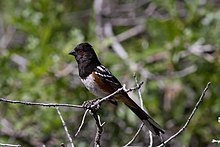
\includegraphics[width=\picwidth]{images/spotow.jpg}}
            \hbox{\tiny Spotted towhee}}\\
    \end{tabular}}
\end{frame}

\begin{frame}
    \frametitle{Method}
        \centering{
\includegraphics[width=.3\textwidth]{images/pytorch.png}}
        \vfill
        \centering{
\includegraphics[width=\textwidth]{images/model.pdf}}
\end{frame}

\begin{frame}
    \frametitle{Results}
    \begin{figure}
        \centering{\includegraphics[height=.8\textheight]{images/confusion.pdf}}
        \caption{Confusion matrix at epoch 4096.}
    \end{figure}
\end{frame}
\begin{frame}
    \frametitle{Results}
    \begin{figure}
        \centering{\includegraphics[height=.6\textheight]{images/error.pdf}}
        \caption{Error percentage. Probability I am guessing $\approx 10^{-84}$}
    \end{figure}
    \centering{checkout the code on \url{github}}
\end{frame}


\end{document}
